\documentclass{beamer}
\usepackage{graphicx}
\usepackage{listings}
\usepackage{kotex}

\usetheme{Berlin}

\title{Form과 Method, 헤더}
\author{허강준}
\institute{충남대학교 정보보호동아리 ARGOS}
\date{2021. 04. 10}

\begin{document}

\begin{frame}
    \begin{center}
        
\includegraphics[height=1.5cm]{../Images/logo.png}
    \end{center}

    \maketitle
\end{frame}

\section{Form \& HTTP Method}
    \begin{frame}{Review: HTTP 패킷의 구조}
        \begin{itemize}
            \item 패킷 = 헤더 + 본문(Body)
        \end{itemize}
        \begin{columns}
            \begin{column}{.5\textwidth}
                \begin{center}
                    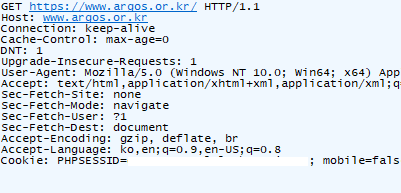
\includegraphics[width=\textwidth]{Images/request_http.png} 
                \end{center}
                
                \begin{itemize}
                    \item 요청 패킷 (GET)
                \end{itemize}                
            \end{column}
            \begin{column}{.5\textwidth}
                \begin{center}
                    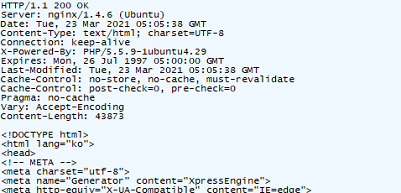
\includegraphics[width=\textwidth]{Images/response_http.png} 
                \end{center}
                \begin{itemize}
                    \item 응답 패킷
                \end{itemize}
            \end{column}
        \end{columns}
    \end{frame}

    \begin{frame}{HTML Form 태그}
        \begin{itemize}
            \item Form: 서식
            \item 회원가입, 로그인, 게시글 작성, 검색창, 등등...
            \item 사용자와 서버를 연결해주는 UI(User Interface)를 구성함
            \item 입력창, 체크박스, 버튼 등등...
        \end{itemize}
        \vspace{0.5cm}
        \begin{columns}
            \begin{column}{0.3\textwidth}
                
\includegraphics[width=\linewidth]{Images/naver_login.png}
            \end{column}
            \begin{column}{0.3\textwidth}
                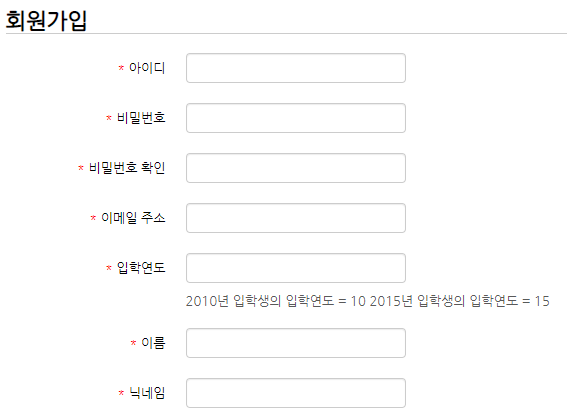
\includegraphics[width=\linewidth]{Images/argos_join.png}
            \end{column}
            \begin{column}{0.3\textwidth}
                
\includegraphics[width=\linewidth]{Images/google.JPG}
            \end{column}
        \end{columns}
    \end{frame}

    \begin{frame}{HTML Form 태그}
        
\includegraphics[width=\linewidth]{Images/form_tag.png}
        \vspace{0.3cm}
        \begin{itemize}
            \item action: 폼 데이터가 전송될 위치(주소)
            \item method: 폼 데이터를 전송하는 방법(Method)
            
            GET, POST, PUT, DELETE 등.. (뒤에 자세히 설명)
        \end{itemize}
    \end{frame}

    \begin{frame}{HTML Form Input 태그}
        
\includegraphics[width=\linewidth]{Images/form_tag.png}
        \vspace{0.3cm}
        \begin{itemize}
            \item type: Input 태그의 종류
            \item name: 서버로 전송될 값의 "이름"
            \item value: 서버로 전송될 값
        \end{itemize}
    \end{frame}

    \begin{frame}{HTML Form Input: text \& password}
        \begin{columns}
            \begin{column}{0.35\linewidth}
                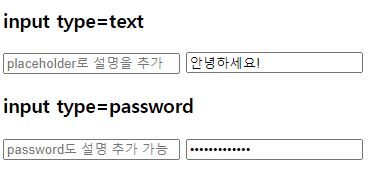
\includegraphics[width=\linewidth]{Images/input_text_password.JPG}
            \end{column}
            \begin{column}{0.65\linewidth}
                \begin{itemize}
                    \item 키보드로 값을 입력받는 폼 요소
                    \item \texttt{type=password} 사용시 입력 내용을 숨길 수 있음
                    \item \texttt{placeholder} 속성 사용시 비어있는 칸에 설명 추가 가능
                \end{itemize}
            \end{column}
        \end{columns}
    \end{frame}

    \begin{frame}{HTML Form Input: checkbox \& radio}
        \begin{columns}
            \begin{column}{0.35\linewidth}
                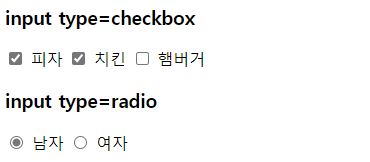
\includegraphics[width=\linewidth]{Images/input_check_radio.JPG}
            \end{column}
            \begin{column}{0.65\linewidth}
                \begin{itemize}
                    \item 여러개 선택 vs 한개만 선택
                    \item \texttt{radio}의 경우 같은 \texttt{name} 끼리는 하나만 선택 가능
                    \item \texttt{checkbox}와 같이 여러개 선택하는 경우 \texttt{name}에 \texttt{[]} 추가하여 배열로 넘기도록 해야함
                    \item 체크된 항목의 \texttt{value}만 서버로 전송됨 (중요)
                \end{itemize}
            \end{column}
        \end{columns}
    \end{frame}

    \begin{frame}{HTML Form Input: select}
        \begin{columns}
            \begin{column}{0.35\linewidth}
                
\includegraphics[width=\linewidth]{Images/select_tag.JPG}
            \end{column}
            \begin{column}{0.65\linewidth}
                \begin{itemize}
                    \item 여러 항목중에서 하나 선택
                    \item \texttt{<input>} 이 아닌 \texttt{<select>} 태그를 사용
                    \item 선택 사항은 \texttt{<select>}, \texttt{</select>} 사이에 \texttt{<option>} 태그로 정의
                    \item 미리 선택되게 하고 싶으면 해당 \texttt{<option>} 태그에 \texttt{selected} 설정
                \end{itemize}
            \end{column}
        \end{columns}
    \end{frame}

    \begin{frame}{HTML Form Input: select}
        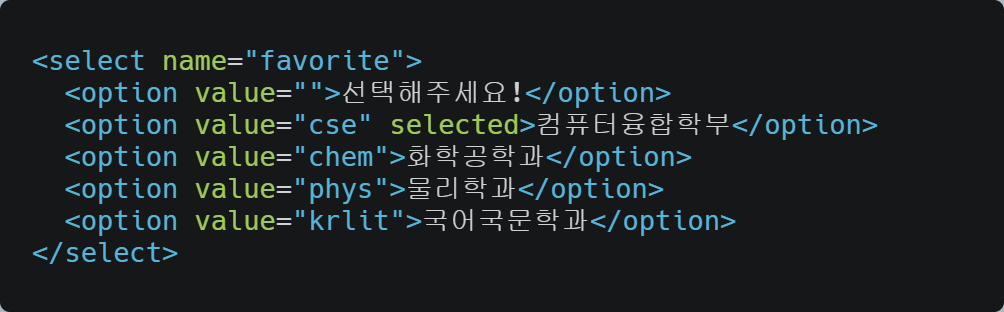
\includegraphics[width=\textwidth]{Images/select_sample.png}
    \end{frame}

    \begin{frame}{HTML Form Input: textarea}
        \begin{columns}
            \begin{column}{0.35\linewidth}
                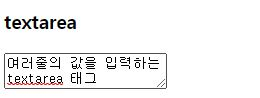
\includegraphics[width=\linewidth]{Images/textarea_tag.JPG}
            \end{column}
            \begin{column}{0.65\linewidth}
                \begin{itemize}
                    \item \texttt{text} 나 \texttt{password}와 비슷하지만 여러줄 입력 가능
                    \item \texttt{<textarea>} 태그 사용
                    \item 값은 \texttt{<textarea>}와 \texttt{</textarea>} 사이에 입력
                \end{itemize}
            \end{column}
        \end{columns}
    \end{frame}

    \begin{frame}{HTML Form Input: submit}
        \begin{columns}
            \begin{column}{0.35\linewidth}
                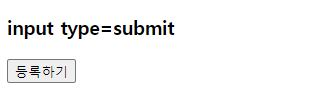
\includegraphics[width=\linewidth]{Images/submit_tag.JPG}
            \end{column}
            \begin{column}{0.65\linewidth}
                \begin{itemize}
                    \item \texttt{text} 나 \texttt{password}와 비슷하지만 여러줄 입력 가능
                    \item \texttt{<textarea>} 태그 사용
                    \item 값은 \texttt{<textarea>}와 \texttt{</textarea>} 사이에 입력
                \end{itemize}
            \end{column}
        \end{columns}
    \end{frame}

\section{HTTP Method}

    \begin{frame}{Method? GET? POST? ???}
        \begin{itemize}
            \item Method: 특정 자원(리소스) 에 대한 요청을 처리하는 방법(Method)
            \item GET: 자원에 대한 "표현" 요청
            \item POST: 특정 자원에 대한 "전송" 요청
            \item PUT: 특정 자원에 대한 "변경" 요청
            \item DELETE: 특정 자원에 대한 "제거" 요청
        \end{itemize}
        \vspace{1cm}
        \tiny{https://developer.mozilla.org/en-US/docs/Web/HTTP/Methods}
    \end{frame}

    \begin{frame}{HTTP GET}
        \begin{itemize}
            \item 자원에 대한 "표현" 요청
            \item 주소에 데이터를 삽입함
            
            http://example.com/index.php?n=example
            \item 여러 데이터의 경우 \& 를 이용하여 연결
            
            http://example.com/index.php?n=example\&n2=example2
            \item 주로 검색창이나 글 읽기 등에 사용
            \item 구현이 간편하나 데이터가 주소에 그대로 표현되므로 보안이 중요하면 사용 금지
        \end{itemize}
    \end{frame}

    \begin{frame}{HTTP GET in PHP}
        \begin{itemize}
            \item \texttt{\$\_GET} 은 GET으로 전달받은 데이터를 보관하는 "배열"
            \item \texttt{\$\_GET["name"]} 식으로 전달된 데이터를 사용할 수 있음
        \end{itemize}
    \end{frame}

    \begin{frame}{HTTP GET in PHP}
        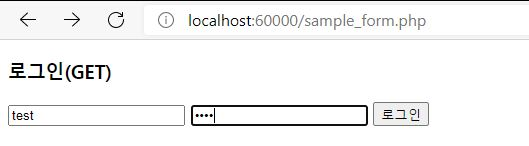
\includegraphics[width=\linewidth]{Images/login_form_get.JPG}
        \vspace{0.8cm}
        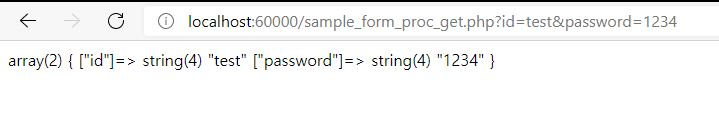
\includegraphics[width=\linewidth]{Images/login_form_get_result.JPG}
    \end{frame}

    \begin{frame}{HTTP POST}
        \begin{itemize}
            \item \texttt{\$\_POST} 는 GET으로 전달받은 데이터를 보관하는 "배열"
            \item 마찬가지로 \texttt{\$\_POST["name"]} 식으로 전달된 데이터를 사용할 수 있음
        \end{itemize}
    \end{frame}

    \begin{frame}{HTTP POST in PHP}
        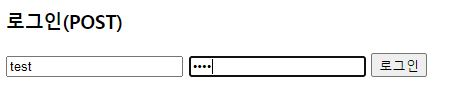
\includegraphics[width=\linewidth]{Images/login_form_post.JPG}
        \vspace{0.8cm}
        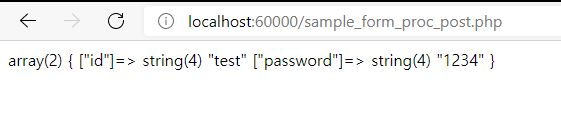
\includegraphics[width=\linewidth]{Images/login_form_post_result.JPG}
    \end{frame}

    \begin{frame}{Request: GET vs POST}
        \begin{columns}
            \begin{column}{0.5\linewidth}
                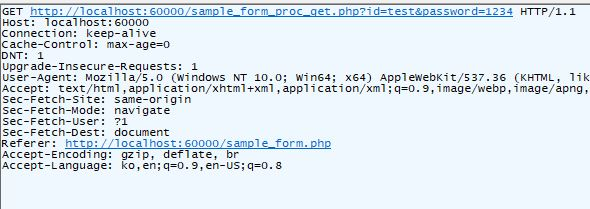
\includegraphics[width=\linewidth]{Images/get_packet.JPG}
            \end{column}
            \begin{column}{0.5\linewidth}
                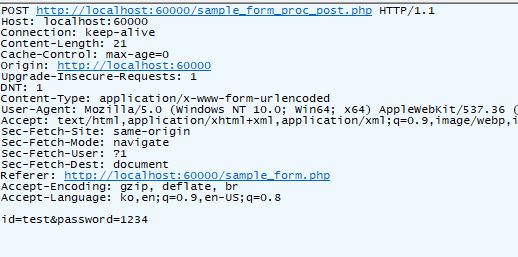
\includegraphics[width=\linewidth]{Images/post_packet.JPG}
            \end{column}
        \end{columns}
    \end{frame}

\section{Header}
    \begin{frame}{Header in Packet}
        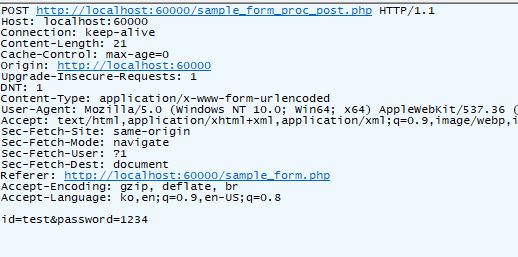
\includegraphics[width=\linewidth]{Images/post_packet.JPG}
    \end{frame}

    \begin{frame}{Header in Packet}
        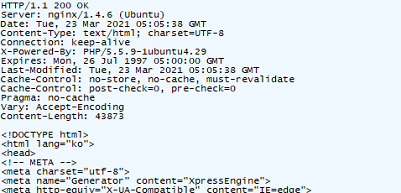
\includegraphics[width=\linewidth]{Images/response_http.png}
    \end{frame}

    \begin{frame}{Header 다시보기}
        \begin{itemize}
            \item HTTP 패킷은 헤더 + 본문(바디)로 이루어짐
            \item 통신을 요청하는 클라이언트나 서버, 혹은 전송되는 데이터에 대한 메타데이터
            \item 헤더와 바디는 헤더 이후의 빈 줄 하나로 구분됨
            \item 바디는 있을수도 없을 수도 있음
        \end{itemize}
    \end{frame}

    \begin{frame}{Request: User-Agent}
        \begin{itemize}
            \item 현재 접속중인 브라우저의 종류를 표현하는 헤더
            \item IE인지, 크롬인지, 사파리인지, 파이어폭스인지, PC인지 모바일인지에 따라 그 내용이 다름
            \item 구현에 따라 전송하지 않도록 할 수 있음
            \item 사용자의 환경에 대한 가장 자세한 정보이므로 여러모로 활용 가능
        \end{itemize}
    \end{frame}

    \begin{frame}{Request/Response: Content-Type}
        \begin{itemize}
            \item 전송되는 데이터의 종류를 표현하는 헤더
            \item 요청/응답 양쪽에서 전송/활용할 수 있음
            \item 값은 MIME이라는 프로토콜을 따름
        \end{itemize}
    \end{frame}

    \begin{frame}{Request/Response: Content-Type - MIME}
        \begin{itemize}
            \item Multipurpose Internet Mail Extensions
            \item 음악, 사진, 영상 등등의 데이터를 간결하게 표현하기 위한 형식
            \item 표준이므로 웬만한 브라우저 등에서 호환 가능
            \item \small{https://www.iana.org/assignments/media-types/media-types.xhtml}
        \end{itemize}
    \end{frame}

    \begin{frame}{Request/Response: Content-Type - MIME}
        \begin{itemize}
            \item 이미지: \texttt{image/bmp, image/jpeg, image/png ...}
            \item 음악: \texttt{audio/mpeg, audio/ogg, ...}
            \item 영상: \texttt{video/mp4, ...}
        \end{itemize}
    \end{frame}

    \begin{frame}{X-Powered-By, Server}
        \begin{itemize}
            \item 프로그램을 구현하는데 사용한 언어, 프레임워크, 서버 데몬의 종류를 표현하는 헤더
            \item 프로그램 구현에 거의 사용될 필요가 없고, 전송해봐야 사용자에게 별다른 영향을 주지 않음
            \item 오히려 Banner Grabbing에 활용될 수 있으므로 설정을 통해 제거하는게 바람직
        \end{itemize}
    \end{frame}
\section{마무리}
    \begin{frame}{PHP에서 디버깅}
        \begin{itemize}
            \item \texttt{var\_dump} 함수는 인자로 넘어온 값의 내부 표현을 출력해줌
            \item 단순 변수, 배열, 객체 등등의 타입, 값을 출력
        \end{itemize}
        \vspace{0.4cm}
        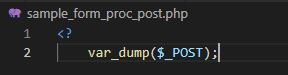
\includegraphics{Images/sample_form_post_source.JPG}
        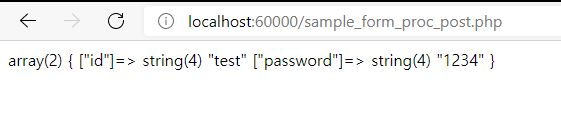
\includegraphics[width=\linewidth]{Images/login_form_post_result.JPG}
    \end{frame}
    \begin{frame}{실습: PHP Calculator}
        \begin{itemize}
            \item 폼 POST 요청을 사용하여 간단한 계산기를 구현해보세요.
            \item 파일명은 \texttt{calculator.php}와 \texttt{calculator\_proc.php}를 사용할 것
            \item 덧셈, 뺄셈, 나눗셈, 곱셈이 가능해야합니다!
            \item 기한: 다음주 활동시간까지
            \item 선택사항1: CSS 등을 사용해서 예쁘게 만들어보세요!
            \item 선택사항2: 굳이 \texttt{calculator\_proc.php}를 사용할 필요가 있을까요?
        \end{itemize}
    \end{frame}


    \begin{frame}{질문?}

    \end{frame}

\end{document}